\documentclass{article}
\usepackage{tikz}
\begin{document}
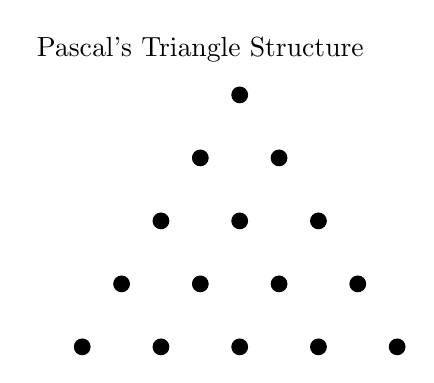
\begin{tikzpicture}
\foreach \i in {1,...,5} {
    \foreach \j in {1,...,\i} {
        \node[draw, circle, inner sep=2pt, fill=black] at (\j - \i/2, -\i*0.8) {};
    }
}
\node[above] at (0, -0.5) {Pascal's Triangle Structure};
\end{tikzpicture}
\end{document}